\chapter{二次函数}
\label{ch: Quadratic Function}

让我们重新回顾一下IGCSE当中的内容

\section*{学习目标}
\begin{todolist}
	\item 掌握完全平方公式,使用配方法对二次多项式进行化简 $ax^2+bx+c$
	\item 推导二次方程$ax^2+bx+c$的\gls{discriminant},并且用判别式确定二次方程\gls{root}的个数
	\item 推导二次方程的\gls{quar form}
	\item 掌握二次函数的图像,包括开口方向,\gls{sym axis}等
	\item 用各种方法求算二次方程,包括配方法,求根公式法,因式分解法,图像法
	\item 求解二次不等式
	\item 解决含有线性和抛物线的方程组
	\item 结合其他代数运算,识别变形的二次方程,并求解
\end{todolist}
\clearpage

\section{二次方程}
\label{sec:Quadratic Equation}
二次方程是形如:
\[
	ax^2+bx+c=0 \qquad ax^2+bx=c \qquad ax^2=bx+c
\]
等包含有$x^2$,$x$ 和常数项的方程,其中,$x^2$项前的\gls{coeff}不能是$0$,否则会变成\gls{lequ}。其他项则可以是$0$。因此$a\neq 0$是唯一的限制条件。

\subsection*{配方}
\label{subsec:Completing the Square}
根据完全平方公式$(\Box+\bigtriangleup )^2=\Box^2+2\cdot \Box \bigtriangleup +\bigtriangleup^2$。将任意含有三项的表达式进行配方调整,其过程与结果如下:
\begin{align*}
ax^2 +bx &+c\\
a\left( x^2+\frac{b}{a}x\right) &+c\\
a\left[ x^2+\frac{b}{a}x+\left(\frac{b}{2a}\right)^2\right]&+c -a\cdot\left(\frac{b}{2a}\right)^2 \\
a\left(x+\frac{b}{2a}\right)^2 &+c-a\cdot \frac{b^2}{4a^2}\\
a\left(x+\frac{b}{2a}\right)^2 &+\frac{4ac-b^2}{4a}
\end{align*}
QED\\

这个技巧是后面\gls{discriminant}和\gls{quar form}的基石,一定要能够自己完全推导出来


\subsection*{二次方程的判别式}
\label{subsec:Discriminant of Quadratic Function}
在刚才的公式中,当表达式变成了方程的时候所有的操作就变成了:
\begin{align*}
ax^2 +bx +c&=0\\
a\left( x^2+\frac{b}{a}x\right)  &=-c\\
a\left[ x^2+\frac{b}{a}x+\left(\frac{b}{2a}\right)^2\right] &=-c +a\cdot\left(\frac{b}{2a}\right)^2 \\
a\left(x+\frac{b}{2a}\right)^2 &=\frac{b^2-4ac}{4a}\\
\left(x+\frac{b}{2a}\right)^2 &=\frac{b^2-4ac}{4a^2}\\
\end{align*}
观察方程两边,LHS是一个整体的平方,必定大于等于0,RHS是一个分式,分母必定是正数,因此该方程针对于$x$可能存在解的前提条件是,RHS的右边也得是一个大于等于0的数字。

因此将
\[
	\Delta = b^2-4ac
\]
计作二次方程的根的\gls{discriminant}。其正负性决定了二次方程是否有根。

其判断结论如下:\\
如果 $\Delta>0$,二次方程有两个不同的实数\gls{root};\\
如果 $\Delta=0$,二次方程有两个相同的实数\gls{root},或者称之为一个实数根;\\
如果 $\Delta<0$,二次方程不存在实数\gls{root},但是可以有一对\gls{conjugate}的复数根


\subsection*{二次方程的求根公式}
\label{subsec:Quadratic Formula}
上方的判断推导如下:
\begin{align*}
	\left(x+\frac{b}{2a}\right)^2 &= \frac{b^2-4ac}{4a^2}\\
	\left(x+\frac{b}{2a}\right)	&= \pm\sqrt {\frac{b^2-4ac}{4a^2}}\\
	x &= \frac{-b}{2a}\pm\sqrt {\frac{b^2-4ac}{4a^2}}\\
	x &= \frac{-b\pm \sqrt{b^2-4ac}}{2a}\\
	x &= \frac{-b\pm \sqrt{\Delta}}{2a}
\end{align*}
该公式被称之为二次方程的\gls{quar form}。需要牢记
\clearpage


\section{二次函数}
\label{sec:Qudratic Function}
对于当我们不拘泥于$ax^2+bx+c$一定要等于$0$时,而是可以用任意值$y$对应之后,二次函数就诞生了。其表达形式为:
\[
	y=ax^2+bx+c
\]

\subsection*{图像}
\label{subsec:Parabola as Its Graph}
利用坐标轴,可以绘制任意二次函数的图像,总结下来无非有这么几点值得关注:
\begin{itemize}
	\item 开口方向与大小
	\item 对称性
	\item \gls{vertex}
	\item $y$轴截距
	\item 是否和$x$轴相交以及通过$\Delta$判断
	\item $x$轴截距以及意义
\end{itemize}

首先,所有的二次函数的图像都是\gls{pwx},如下图所示:
\begin{figure}[H]
\centering
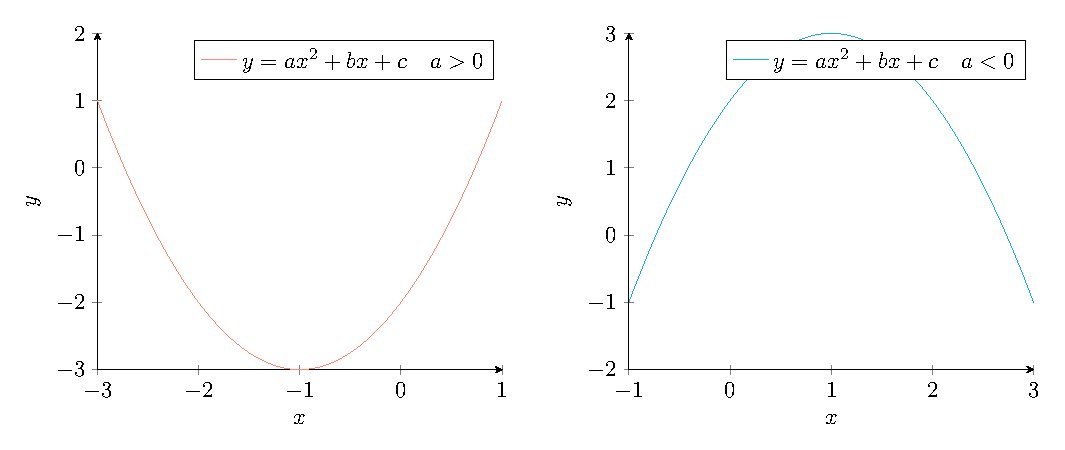
\includegraphics[width=0.9\textwidth]{parabola}
\label{二次函数的两种开口}
\end{figure}

开口的方向只有两种,向上或者向下。判断一句是$a$的正负性。
当$a>0$时,开口朝上;
当$a<0$时,开口朝下;

为什么不提当$a=0$的时候的情况呢?因为在二次函数中作为$x^2$的系数不能是0啊。

其次,抛物线都是对称的,其对称轴为
\[
	x=-\frac{b}{2a}
\]
因为利用配方法可以得到:

\[
	y=\left(x+\frac{b}{2a}\right)^2+\frac{4ac-b^2}{4a^2}\\
\]
由于$\left(x+\frac{b}{2a}\right)$部分只要绝对值一致,其平方必定相等,所以导致两个不同的$x$值,可以得到同样的$y$,这两个点必定关于$-\frac{b}{2a}$对称。

第三点,\gls{vertex}是二次函数图像上只有唯一的函数值的点,同时也是对称轴和函数的交点。因此该点的横坐标为$-\frac{b}{2a}$,将其带入到函数表达式中,得到纵坐标为$\frac{4ac-b^2}{4a}$。标记在一起可得顶点坐标为$\left(-\frac{b}{2a}, \frac{4ac-b^2}{4a}\right)$。 为了便于记忆,我们将该点的坐标计作$(h,k)$在后面的内容中将用到该表达式。

\begin{TaskBox} 
请在刚才的红蓝的二次图像中标记顶点坐标,并判断,当满足何种条件的时候,顶点为二次函数的最高/低点。
\end{TaskBox} 

紧接着,关于\gls{intercept}。由于$y$轴截距必定是当横坐标$x=0$时点,因此直接带入到二次函数的表达式中,$(0,c)$ 就判断出来了。

下一点,\\
如果$\Delta>0$,二次函数会与$x$轴有两个交点;\\
如果$\Delta=0$,二次函数会与$x$轴有相切,产生一个交点;\\
如果$\Delta<0$,二次函数会与$x$轴不会相交。

有没有发现和二次方程的$\Delta$判断非常相像,然而这是为什么呢?看看$x$轴截距的含义就可以了,$x$轴的交点,是指当二次函数的$y=0$的时候,$x$的取值。因此$0=y=ax^2+bx+c$。求解出$x$的值就是之前的二次方程的解。所以,利用之前的手段。如果二次函数图像与$x$轴相交的话,产生的两个截距的坐标分别就必定是
\[
	(x_1,0) \qquad (x_2,0)
\]
这两个值和二次方程的根完全一样。$x_1, x_2=\frac{-b\pm \sqrt{b^2-4ac}}{2a}$。稍后在二次方程的多重形式中,我们会用到。

至此,我们所有的关于二次函数的图像就全部结束了,需要能够根据给定的$a$,$b$, $c$的值,绘制二次函数的函数图像。反过来根据图像也能够求算表达式。

\subsection*{二次的求解方式}
\label{subsec:Ways of Solving Quadratic Equation}
我们又重新看一次二次方程,到目前为止,已经可以产生四种求解的方法,他们分别是:
\begin{itemize}
	\item 配方法
	\item 求根公式法
	\item 因式分解,十字相乘法
	\item 图像法
\end{itemize}

其中图像法就是之前所讨论的,绘制二次函数的图像,寻找其与$x$轴的交点。这种方法实际上和因式分解是完全一致的。因为根据之前所提及的关系,如果一个二次函数与$x$轴产生的两个交点分别为$(x_1,0)$和$(x_2,0)$的话,那么该二次函数的表达式必定可以从$y=ax^2+bx+c$化简为$y=a(x-x_1)(x-x_2)$。

\begin{TaskBox}  %这个会有一点问题
利用$x_1,x_2=\frac{-b\pm\sqrt{\Delta}}{2a}$ 验证刚才所说的正确性
\end{TaskBox}

所以,对于一个普通形式的二次函数$y=ax^2+bx+c$ 或者二次方程$0=ax^2+bx+c$。我们可以尽量地去尝试将这些方程改写为两个因式相乘的形式。这样求算方程的解,或者图像的交点就非常简单,寻找该因式分解过程的方法叫做十字交叉法。
以这条题目为例子:
\[
	60x^2-217-30=0
\]
首先,可以将$60x^2$拆分为$15x$和$4x$;\\
然后,将$-30$拆分为$-2$和$+15$;\\
接着,列出如下的形式
\[
\begin{matrix}
15x & -2\\
4x & +15
\end{matrix}
\]
将\textbf{对角线相乘}去验证是否可以得到中间的一次项$-217x$。实际上就是展开$(15x-2)\cdot(4x+15)$。非常幸运,我们的尝试是正确的。因此\\
最后,化简成为$60x^2-217-30=(15x-2)\cdot(4x+15)=0$。那么该方程的解就是$x=\frac{2}{15}$或者$-\frac{15}{4}$

这个方法的局限性非常大,但是考试当中由于基本是整数,且$\Delta$一般是一个平方数,因此基本上还是凑得出来的。

\subsection*{二次函数的等价形式}
\label{subsec:Multiple Equivalent Form of Quadratic Function}
我们似乎看到了三种关于二次函数的形式,他们分别是:
\begin{align*}
 y &= ax^2+bx+c\\
 y &= a\left(x+\frac{b}{2a}\right)^2+\frac{4ac-b^2}{4a}\\
 y &= a\cdot \left(x-\frac{-b+\sqrt{b^2-4ac}}{2a}\right)\left(x+\frac{-b+\sqrt{b^2-4ac}}{2a}\right)
\end{align*}

通过严密的代数推导,这三种形式是完全等价的。
为了方便简洁,后面的两个式子分别用之前我们提到过的顶点坐标和$x$轴截距坐标来表示,可以整理为:
\begin{align*}
 y &= ax^2+bx+c \qquad \text{standard form}\\
 y &= a(x-h)^2+k \qquad \text{vertex form}\\
 y &= a(x-x_1)(x-x_2)\qquad \text{root/factorized form}
\end{align*}

\begin{TaskBox}
请写出$(h,k)$的代数表达式,以及含义;
\tcblower
写出$(x_1,0) \ (x_2,0)$代数表达式,以及含义。
\end{TaskBox} 

在该\href{https://www.desmos.com/calculator/vzy4hytj5j}{desmos}当中有我们所有的推导。

\subsection*{二次不等式}
\label{subsec:Quadratic Inequality}
当我们把二次方程中的等于号替换为不等符号之后,我们得到了形如下方的二次不等式:
\[
	ax^2+bx+c>0 \quad ax^2+bx+c<0 \quad ax^2+bx+c\le 0 \quad ax^2+bx+c\ge0
\]
求解该不等式,其实只需要做好这三件事:\\
1. 求解对应的二次方程$ax^2+bx+c=0$。得到两个解$x_1$和$x_2$(如果有的话)\\
2. 绘制$y=ax^2+bx+c$的图像,标记两个解。根据不等于符号,明确是函数图像的下方还是上方。会和开口方向有关系\\
3. 写出方程的解,通常在两根之间,或者两根之外,以$x_1<x<x_2$ 或者 $x>x_1 \text{ or } x>x_2$的形式出现(假设$x_1$是较小的解)。

如下图所示:
\begin{figure}[H]
\centering
\includegraphics[width=0.4\textwidth]{quarinequ_1}
\includegraphics[width=0.4\textwidth]{quarinequ_2}
\end{figure}

\clearpage

\section{方程式组}
\label{sec:System from Linear and Quadratic Function}
一个二次函数和一个线性函数联立,构成\gls{fcz}。形成如下形式的
\[
\left\{\begin{matrix}
 y=mx+d\\
y=ax^2+bx+c
\end{matrix}\right.
\]

这是非常经典方程式组,几乎就是二次函数届的鸡兔同笼问题。

求解这样的方程组无非两个思路:\\
1. 通过\textbf{替换 Substitution}或者\textbf{消元 Elimination}变成只含有$x$的二次方程:$mx+d=ax^2+bx+c$。然后再求解\\
2. 利用两个函数的图像的\textbf{交点 Intersection}。在IGCSE阶段就是经典的曲线绘图问题。
\clearpage


\section{伪装的二次方程}
\label{sec:Qudratic Equation in Disguise}

任何具有三项的表达式,并且满足次数的平方关系,都可以通过换元法转变为二次方程,因此你可以认为以下的方程就是披着一层羊皮的二次方程。
\[
\begin{matrix} %这里报$$的错需要调整看看
e^{2x}-3e^x-10=0  & \boxed{e^x}^2-3\boxed{e^x}-10=0\\
x^4-5x^2+4=0      & \boxed{x^2}^2-5\boxed{x^2}+4=0\\
6x-\sqrt{x}-1=0   & \boxed{\sqrt{x}}^2-\boxed{\sqrt{x}}-1=0\\
\tan^2 x=1+\tan x & \boxed{\tan x}^2=1+\boxed{\tan x}
\end{matrix}
\]

这些公式当中,右侧盒子中的部分都可以当做整体,换元为$t$,$u$,$y$等其他变量。然后再求算。只不过这一类的换元当中,要关注$e^x$, $x^2$,$\sqrt{x}$的取值范围。

\begin{TaskBox}
分别求算上面方程中$e^x$,$x^2$,$\tan x$的值
\tcblower
再求算出对应的$x$的解
\end{TaskBox}

